\section{Implementação de Hardware}

\subsection{Sensor de Temperatura}

O sensor de temperatura DS18b20 é alimentado pelos pinos de 5V e GND (terra) do microcontrolador. seu sinal de leitura é enviado para uma porta digital, sendo utilizado um resistor de 4,7 k$\Omega$ como pull up, caso exista uma leitura errada do sensor. A figura \ref{fig:micro_temp} ilustra a conexão do microcontrolador com o sensor de temperatura. 


\begin{figure}[h]
    \centering
    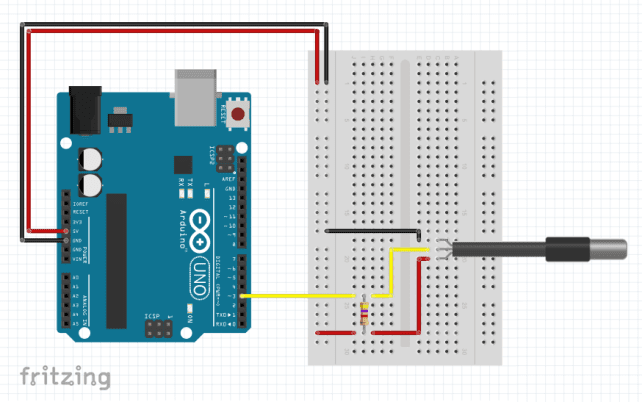
\includegraphics[scale=0.40]{figuras/implementacao/hardware/DSsensor.png}
    \captionsource{Esquema de conexão entre microcontrolador e sensor de temperatura DS18B20.}{https://portal.vidadesilicio.com.br/}
    \label{fig:micro_temp}
\end{figure}


O excerto de código em linguagem Arduino a seguir representa a função utilizada para ler o valor de saída do sensor. A biblioteca OneWire (\url{https://github.com/PaulStoffregen/OneWire}) implementa o protocolo proprietário de comunicação serial da Dallas Semicondutor, fabricante do sensor. Ela é utilizada em conjunto com a biblioteca livre DallasTemperature (\url{https://github.com/milesburton/Arduino-Temperature-Control-Library}) para estabelecer a comunicação com o DS18B20.

\begin{lstlisting}[language=C]

#include <OneWire.h>
#include <DallasTemperature.h>
#define ONE_WIRE_BUS D6

OneWire oneWire(ONE_WIRE_BUS);
DallasTemperature sensors(&oneWire)

void setup() {
    sensors.begin();
}

float readTemperature() {
    return sensors.getTempCByIndex(0);
}

\end{lstlisting}


\subsection{Sensor de pH}

O sensor de pH é conectado a um circuito auxiliar que trata o sinal proveniente da ponta de prova. Esse circuito é conectado aos pinos de 5V e GND do microcontrolador para alimentação, e envia do dado coletado por meio de sinal analógico, como observado na figura \ref{fig:micro_ph}. 


\begin{figure}[h]
    \centering
    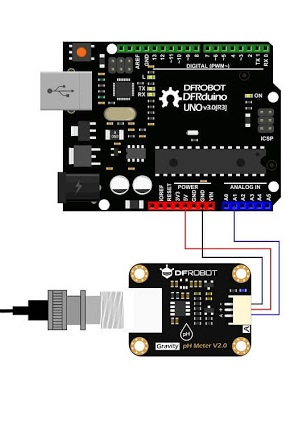
\includegraphics[scale=0.65]{figuras/implementacao/hardware/micro_ph.jpg}
    \caption{Esquema de conexão entre microcontrolador e sensor de pH E-201-C.}
    \label{fig:micro_ph}
\end{figure}


Para utilização desse sensor, é necessário sua calibração, que consiste na medição da tensão de saída do sensor em soluções com diferentes concentrações de \(H^+\) e obtenção de uma equação linear que traduza a voltagem medida em um valor de pH. Para isso utilizadas soluções tampão com pH iguais a 4, 7 e 10. A calibração seguiu o seguinte processo:
\begin{enumerate}
    \item Com a solução de pH igual a 7, ajustar o ganho do circuito (por um potenciômetro) até que a leitura de voltagem seja 2,5 Volts. Essa tensão foi escolhida de forma a coincidir valor médio da tensão de alimentação do circuito com o valor médio da escala de pH;
    \item Capturar a tensão medida nas soluções com pH 4 e 10;
    \item Aplicar regressão linear, minimizando a soma dos erros quadráticos, obtendo a reta que relaciona a tensão medida com o pH da solução
\end{enumerate}


Com os valores obtidos na tabela \ref{tab:calibra_ph}, foi obtida a equação linear \ref{eq:pH}.

\begin{equation}
    pH = 2.0171 \cdot Voltagem + 1.7152
    \label{eq:pH}
\end{equation}


\begin{table}[H]
    \begin{center}
        \begin{tabular}{ |c|c| } 
            \hline
            Voltagem & pH \\
            \hline
            2.50 & 7.0 \\ 
            \hline
            1.20 & 4.0 \\ 
            \hline
            4.16 & 10.0 \\ 
            \hline
        \end{tabular}
        \caption{\label{tab:calibra_ph}Medições de tensão em soluções tampão para calibração do sensor de pH.}
    \end{center}
\end{table}


A leitura do pH medido pelo sensor pelo microcontrolador segue o seguinte algoritmo:
\begin{enumerate}
    \item Valor inteiro entre 0 e 1024 recebido pelo sensor é lido na porta analógica;
    \item Valor lido é convertido em uma diferença de tensão seguindo \(Voltagem = medida \cdot 5 / 1024\);
    \item Diferença de tensão é convertida na leitura de pH seguindo equação linear obtida na calibração do sensor.
\end{enumerate}


% \begin{lstlisting}[language=C]

% int ph_pin = A0;

% float readPH() {
%     int measure = analogRead(ph_pin);
%     double voltage = measure * 5 / 1024;
%     return 2.0171 * voltage + 1.7152;
% }

% \end{lstlisting}

\subsection{Sensor de pressão diferencial para medida de densidade}

A medição de densidade foi implementada indiretamente através do sensor de pressão diferencial MP3V5010DP. Esse sensor é inserido no líquido fermentado através de dois tubos posicionados em uma distância fixa de 18 centímetros. A densidade é inferida através da fórmula: 

\begin{equation}
    \rho = \dfrac{\Delta P}{g \cdot \Delta h}
\end{equation}

O chip Pmod DPG1 se comunica com o microcontrolador através da interface periférica serial (SPI), que é um sistema de comunicação que utiliza as portas: SCK: Serial Clock (output from master), MISO: Master In Slave Out (data output from slave) e SS: Slave Select.

O sensor é alimentado com 3.3 V e é utilizado um conversor de nível lógico bidirecional para converter o sinal digital de 5V para a tensão do sensor. A biblioteca SPI (https://github.com/PaulStoffregen/SPI) foi utilizada para realizar essa comunicação e leitura. O valor recebido pelo microcontrolador é convertido através da fórmula fornecida no datasheet do chip:

\begin{equation}
    \Delta P = \dfrac{\dfrac{value}{4096} - 0.08}{0.08} 
\end{equation}

\subsection{Conexão e Comunicação do Microcontrolador}

Com os sensores propriamente conectados e calibrados, o microcontrolador foi configurado para se conectar à Internet através de conexão \textit{Wi-Fi} e a enviar os dados coletados por meio do protocolo MQTT. O Wemos D1 é controlada pelo módulo ESP8266, de forma que ofereça conectividade \textit{Wi-Fi} nativa. 
A biblioteca ESP8266\textit{Wi-Fi} (\url{https://github.com/esp8266/Arduino/tree/master/libraries/ESP8266WiFi}) foi utilizada para estabelecer a conexão \textit{Wi-Fi}, em conjunto com a biblioteca PubSubClient (\url{https://github.com/knolleary/pubsubclient}) para publicar mensagens e se inscrever em tópicos MQTT. 


% // TODO: Colocar código completo em Apêndice e discutir Fluxo completo aqui


\subsection{Controle de Temperatura}

Um controlador de malha fechada proporcional interativo derivativo (PID) é utilizado para controlar a temperatura do fermentador. Esse método é amplamente utilizado na indústria, possuindo boa precisão e confiabilidade, além de ser facilmente sintonizado. Inicialmente são definidos parâmetros analógicos e depois é criado o controle digital.


Sendo assim, o sistema com a pastilha de Peltier deve retirar do sistema uma quantidade de calor proporcional a essa recebida e gerada para manter uma temperatura estável abaixo do ambiente. Como a quantidade de calor retirada por um Peltier é proporcional a corrente, a tensão fornecida a pastilha é variada através de uma circuito ponte H que tem a sua amplitude de tensão de saída regulada por uma porta PWM.  

\subsubsection{Circuito Ponte H}

O circuito ponte H (figura \ref{fig:ponte_h}) permite que a amplitude e sentido da tensão de entrada da pastilha de Peltier seja controlado digitalmente por um sinal PWM (Pulse Width Modulation) do microcontrolador. No Software embarcado, um valor entre 0 e 255 é utilizado para definir o duty cycle da onda quadrada do sinal PWM, como exemplificado na figura \ref{fig:pwm}. 


\begin{figure}[H]
    \centering
    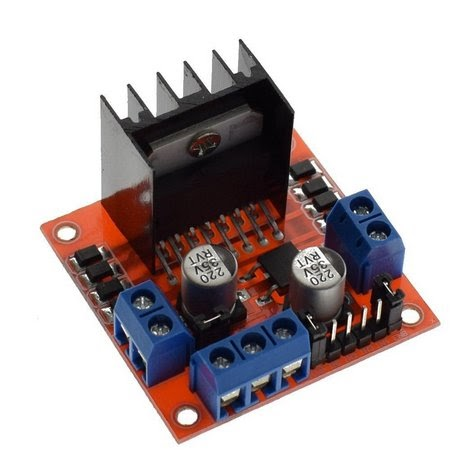
\includegraphics[scale=0.35]{figuras/implementacao/hardware/ponte_h.jpg}
    \captionsource{Modelo ponte H - L298N.}{https://mercadolivre.com.br/}
    \label{fig:ponte_h}
\end{figure}

\begin{figure}[H]
    \centering
    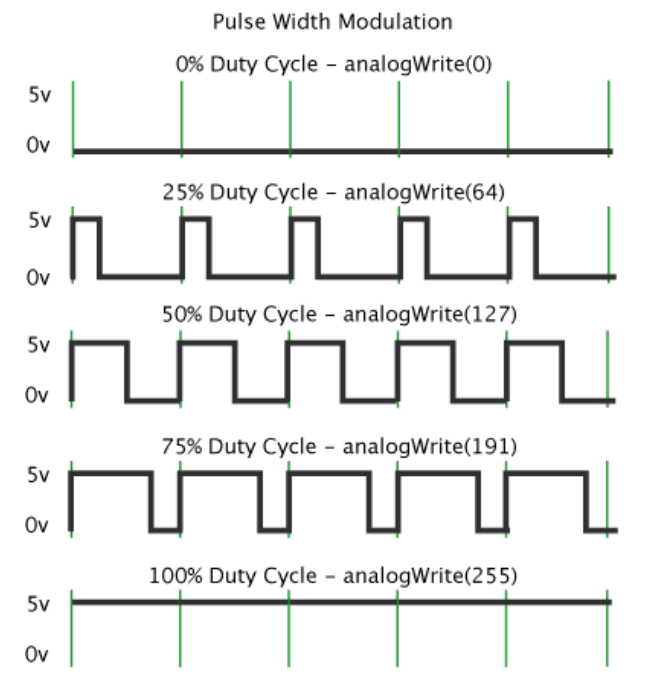
\includegraphics[scale=0.30]{figuras/implementacao/hardware/pwm.png}
    \captionsource{Onda quadrada do sinal PWM para alguns valores especificados no microcontrolador.}{https://www.arduino.cc/}
    \label{fig:pwm}
\end{figure}


\subsubsection{Montagem do Dispositivo}

Com as definições de controle discutidas, foi projetado o dispositivo da figura \ref{fig:dispositivo_term}, em escala aproximada. O dispositivo pode ser dividido em três partes descritas a seguir:

\begin{enumerate}
    \item Parte quente : Essa parte é ligada na face quente da pastilha e é formada por uma ventoinha e um dissipador de calor. Uma boa dissipação de calor garante uma melhor eficiência da partilha e permite que ela forneça quantidades de calor maiores para o sistema;
    \item Pastilha de Peltier: Pastilha que recebe a corrente e transforma energia elétrica em térmica. A face quente e face fria são isoladas por material isolante térmico, que ajuda na não interferência entre as partes e melhora a eficiência do sistema;
    \item Parte fria: essa parte é ligada na face fria da pastilha. Ela retira calor do sistema através de uma placa de cobra e barras de aço inox. Apesar do cobre ter uma condutividade térmica melhor, o aço inox foi escolhido para fazer a transmissão para o mosto + leveduras, por não interferir no seu gosto na exposição de pHs menores. 
\end{enumerate}


\begin{figure}[H]
    \centering
    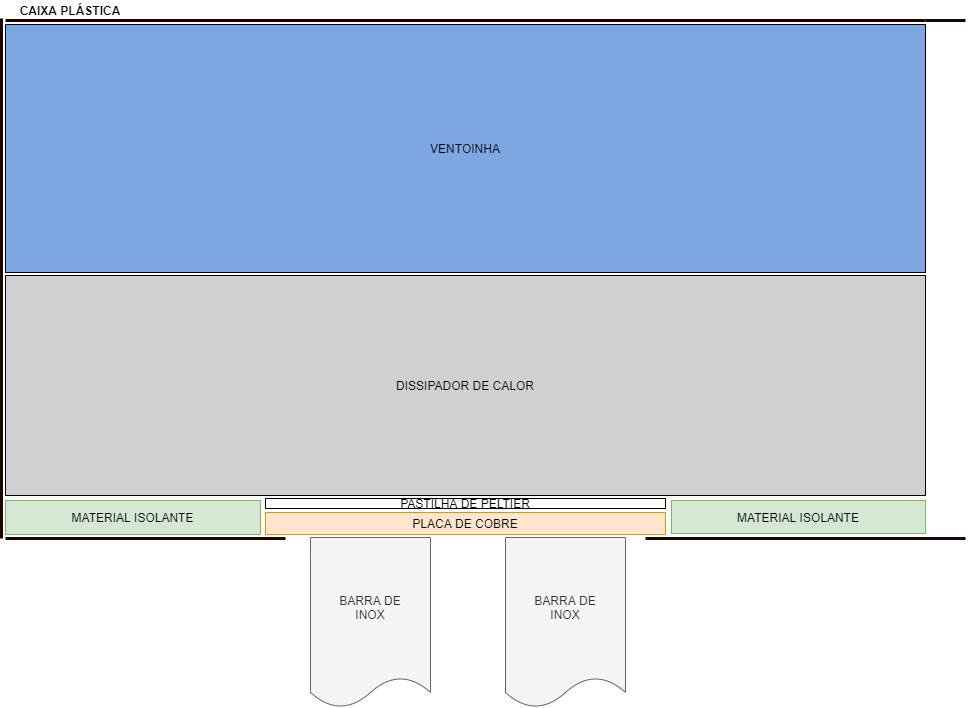
\includegraphics[scale=0.45]{figuras/implementacao/hardware/montagem.png}
    \captionsource{Esquema do perfil do dispositivo controlador de temperatura, escala aproximada.}{Autores}
    \label{fig:dispositivo_term}
\end{figure}

